\chapter{State of the Art and Related Research} % Main chapter title
\label{Chapter2}

\section{Energy consumption measurement and efficiency on data center level}

Energy consumption and efficiency on a data center level has been well-studied to the point where various Literature reviews were published\parencite{long2022review}\parencite{jin2020review}. The bigger part of this research is focused on the data center infrasturture (cooling and power), and with good reason, as the data center infrastructure is responsible for a large part of the energy consumption. While a large number of coarse-, medium- and fine-grained metrics for data center energy consumption exist, most data center operators have focused on improving coarse-grained mertrics (especially the \textit{Power Utilization Effectiveness, PUE}) with improvements to infrastructure. This has resulted in a PUE of 1.1 or lower in some cases\parencite{uptime2023pue}. Meanwhile, server energy efficiency has substantially improved, especially for parial load and idle power\parencite{tropgen202416}. This has allowed data center operators to improve energy efficiency by simply installing more efficient cooling and power systems and servers. Fine-grained metrics such as server component utilization rates or speed were generally not used in the context of energy efficiency, but rather as performance metrics to ensure customer satisfaction.

\section{Energy consumption measurement on a server level}

As a result of the energy efficiency improvements of both data center infrastructure and server hardware mentioned in the previous section, a shift has started towards evaluating the actual server load energy efficiency. Efficiency gains on this level compound into further gains at the data center level. The method of resource-sharing of modern cloud computing (and especially the use of containers) have created great opportunities for server workload optimitation for energy efficiency, which in turn require power consumption measurements for evaluation. In the context of containers on multi-core processors, measuring the energy consumption of the entire server is insufficient, since it does not allow the attribution of consumped energy to specific containers or processes. While component-level power measurements provide finer measurements that could theoretically be modelled to display container energy consumption, they drastically raise the complexity for a number of reasons:

\begin{itemize}
    \item Component-level energy consumption measurement without external tools is far from easy. While some components provide estimation models (e.g. Intel RAPL or Nvidia SMI), others can only be estimated using their performance metrics. This will invariably lead to large measurement uncertainties, especially with the component hardware differences between generations and manufacturers.
    \item The problem of attributing measured or estimated energy consumption to individual containers is in itself non-trivial: It not only requires a fine-grained time synchronization of energy consumption and used container resources due to the fast-switching nature most server components during any sort of multitasking.
    \item A deep understanding of dynamic or static energy consumption is required: Depending on the energy consumption attribution model, a container might not only account the energy it actively used, but potentially also account for a fraction of the energy consumed for any shared overhead such as shared hardware components, or system resources (such as the Kubernetes system architecure). This idea can be further extended: containers could potentially be penalized for any unused server resources, as these unused capacity still consume energy. These different attribution models lead to a larger debate about the goals of the measurements.
    \item Any server-level power models used to estimate the relation of individual component energy consumption suffers from the varity of different server configurations due to server specialization, such as Storage-, GPU-, or Memory-optimized servers.
    \item 
\end{itemize}

The following sections of this chapter aim to present the current state-of-the-art in the various fields of research of the problem domains listed above. 

xxxxxxxxxxxxxxxxxxxxxxxxxxxxxxx
here, a sentence will introduce the subsections:
\begin{itemize}
    \item Hardware components: CPU / RAM / SoC / GPU / \dots
    \item 
\end{itemize}
xxxxxxxxxxxxxxxxxxxxxxxxxxxxxxx

Finally, section xxxxxxxxxxxxxxxxxxxxxxxxxxxx aims to give an overview of the currently existing implementations of software-based container-level energy consumption estimation.

\section{Overview of Power Data collection}

In a systematic review cloud servers power models, Lin et al\parencite{lin2020taxonomy} categorize power collection methods into 4 categories:
\begin{table}[h]
    \tiny
    \begin{tabular}{ |p{2cm} | p{2cm} | p{2.5cm} | p{1.2cm} | p{2cm} | p{1.5cm} |} 
        \hline
        \textbf{Key} & \textbf{Value} & \textbf{Description} & \textbf{Deployment Difficulty} & \textbf{Data Granularity} & \textbf{Data Credibility}\\
        \Xhline{1.5pt}
        Based on instruments & Installation of extra devices & Bare-metal machines & Easy & Machine Level & Very high \\
        \hline
        Based on dedicated aquisition system & Specialized systems & Specified models of machines & Difficult & Machine or component-level & High \\
        \hline
        Based on software monitoring & Build-in power models & Bare-metal and virtual servers & Moderate & Machine, component, or VM level & Fair \\
        \hline
        Based on simulation & System simulation & Machine, component or VM level & Easy & Machine, component, or VM level & Low\\
        \hline
    \end{tabular}
    \caption[Comparison of power collection methods for cloud servers]{Comparison of power collection methods for cloud servers}
    \label{tab:power_collection_methods}
\end{table}



\subsection{Instrument-based power data aquisition}

Instrument-based Data collection aquisition produces the hightest data credibility at a low granularity: These devices, installed externally (measuring the power supplied to the PDU) or internally (measuring the power flow between the PDU and motherboard) have been the source of information for a number of studies. The approach to simply measure electric power at convenient hardware locations using dedicated equipment can of course be extended to provide additional granularity: For example, Desrocher et al\parencite{desrochers2016validation} custom-created a DIMM extender custom-fitted with Hall-sensor resistors and a linux measurement utility to measure power consumed by a DIMM memory module at 1kHz sampling rate using a \textit{WattsAppPro?} power meter and a \textit{Measurment Computing USB.1208FS-Plus} data aquisition board.

This of course highlights a fundamental truth of instrument-based data collection: While it is possible to implement a measuring solution that provides high-granular and high-sampling rate power data, it is paired with an immense effort since solutions like this are not provided off-the-shelf. Unsuprisingly, this is most valuable for benchmarking or validation (Desrochers used this setup to validate Intel RAPL DRAM power estimations on three different systems). However, this methodology is (currently) unsuitable for deployment to data center servers due to its bad scalability and prohibitive costs. Hence, the primary role of instrument-based power data aquisiton is as a benchmarking and validation tool for research and development.

\subsection{Dedicated Aquisition systems}
\subsubsection{BMC Devices, IPMI and Redfish}
Some manufacturers have developed specialized power data aquisition systems for their own server products. The baseboard management controller (BMC) is a typical dedicated aquisition system usually integrated with the motherboard, usually as part of the intelligent platform management interface (IPMI)\parencite{lin2020taxonomy}. It can be connected to the system bus, sensors and a number of components to provide power and temparature information about the CPU, memory, LAN port, fan, and the BMC itself. Some comprehensive management systems such as Dell iDRAC or Lenovo xClarity have been further developed to provide high-quality, fine-grained power data due to their close interoperation between system software and underlying hardware. BMC devices on modern servers often offer IPMI- or Redfish interfaces. While these interfaces use the same physical servers, their implementation differ significantly, where Redfish generally offers higher accuracy (e.g through the use of higher-bit formats, whereas IPMI often uses 8-bit raw numbers).

In the context of container power consumption estimation, IPMI-implementations occupy an interesting role. In 2016, Kavanagh et al\parencite{kavanagh2016accuracy} found the accuracy of IMPI power data to be relatively inaccurate when compared with an external power meter, mainly due to the large measurement window size of 120 to 180 seconds and the inaccurate assessment of the idle power. They concluded that IMPI power data was still useful when a longer averaging window was used, and the initial datapoints discounted. In a later study, they suggest combining the measurements of IPMI and Intel RAPL (which they find to underestimate the power consumption) for a reasonable approximation of true measurement\parencite{kavanagh2019rapid}. Kavanagh's findings have been cited in various studies, often to negate the use of IPMI for power measurement. When used, it sometimes is chosed because it was the "simplest power metric to read"\parencite{white2020monitoring} in the context of entire data centers.

Redfish is a modern Out-of-band Management System, first released in 2015 explicitely to replace IPMI \parencite{thomas-krenn-redfish}. It uses a RESTful API and JSON data format, making queries with code easier. In 2019, Wang et al\parencite{wang2019empirical} directly compared IPMI and redfish power data to a reading of a high accuracy power analyzer, and found Redfish to be more accurate than IPMI, with a MAPE of 2.9\%, while also finding a measurement latency of about 200ms. They also found measurements to be more accurate in higher power ranges, which they attribute to the improved latency.

In conclusion, BMC power data aquired over Redfish provides a simple simple and comparatively easy way to measure system power based on various physical system sensors. Its biggest strenght lies in easy implementation and general availability. In the context of container energy consumption, BMC power data lacks the short sampling rates necessary to measure a a highly dynamcic container setup, but can prove useful as a validation or cross-reference dataset for longer intervals exceeding 120 seconds. Unfortunately, the data quality of BMC power data depends on the actual system, and power models can be significantly improved by initial calibration with an external power measurement device\parencite{kavanagh2016accuracy}.

\subsection{Power Monitoring Counters: Intel RAPL}

Intel Running Average Power Level (RAPL) is a Power Monitoring Counter (PMC)-based feature introduced by Intel and provides a way to monitor and control the energy consumption of various components within their processor package\parencite{projectexigence_rapl}. An adaptation of RAPL for AMD processors uses largely the same mechansms and the same interface\parencite{amd_energy}, although it provides less information than Intel's RAPL, providing no DRAM energy consumption\parencite{schone2021energy}.

Intel RAPL has been used extensively in research to measure energy consumption\parencite{kennes2023measuring} despite some objections about its accuracy, which will be discussed sections~\ref{sec:raplvalidation} and ~\ref{sec:rapllimitations}. The general concencus is that RAPL is \textit{good enough} for most scientific work in the field of server energy consumption and efficiency. As Raffin et at\parencite{raffin2024dissecting} point out, it is mostly used \textit{like a black box without deep knowledge of its behavior}, resulting in implementation mistakes. For this reason, the next section~\ref{sec:raplmethodology} presents an overview of the RAPL fundamentals.Finally, section~\ref{sec:rapltools} discusses the currently available RAPL-based tools.

\subsubsection{RAPL measuerment methods}
\label{sec:raplmethodology}
This subsection provides an overview of how RAPL works and is used. It is based on the Intel rchitectures Software Developer’s Manual\parencite[Section 16.10]{intel-sdm} and the works of Raffin et al \parencite{raffin2024dissecting} (2024) and Schöne et al \parencite{schone2024energy} (2024).

Running Average Power Limit (RAPL) is a power management interface in Intel CPUs. Apart from power limiting and thermal management, it also allows to measure the energy consumed by various components (or \textit{domains}). These domains individual CPU cores, integrated graphics (in non-server CPUs) and DRAM, as well as \textit{package}, refering to the whole CPU die. While it initially used models to estimate energy use\parencite{hackenberg2015energy}, it now uses physical measurements. The processor is divided into different power domains or "planes", representing specific components, seen in figure~\ref{fig:rapl_domains}. Notably, not all domains are present in all systems: Both client-grade systems feature the \textit{Package} and \textit{PP0 core} domains, server grade processors typically don't show the \textit{PP1 uncore}-domain typically used for integrated GPUs, and client-grade processors don't show the \textit{DRAM} domain. The \textit{PSYS} domain for the "whole machine" is ill defined and only exists on client-grade systems. In an experiment with recent Lenovo and Alienware laptops, Raffin et al found that the \textit{PSYS} domain reported the total consumption of the laptop, including display, dedicated GPU and other domains. Regardless, this thesis will focus on the RAPL power domains available to server-grade processors.

\begin{figure}[ht]
    \centering
    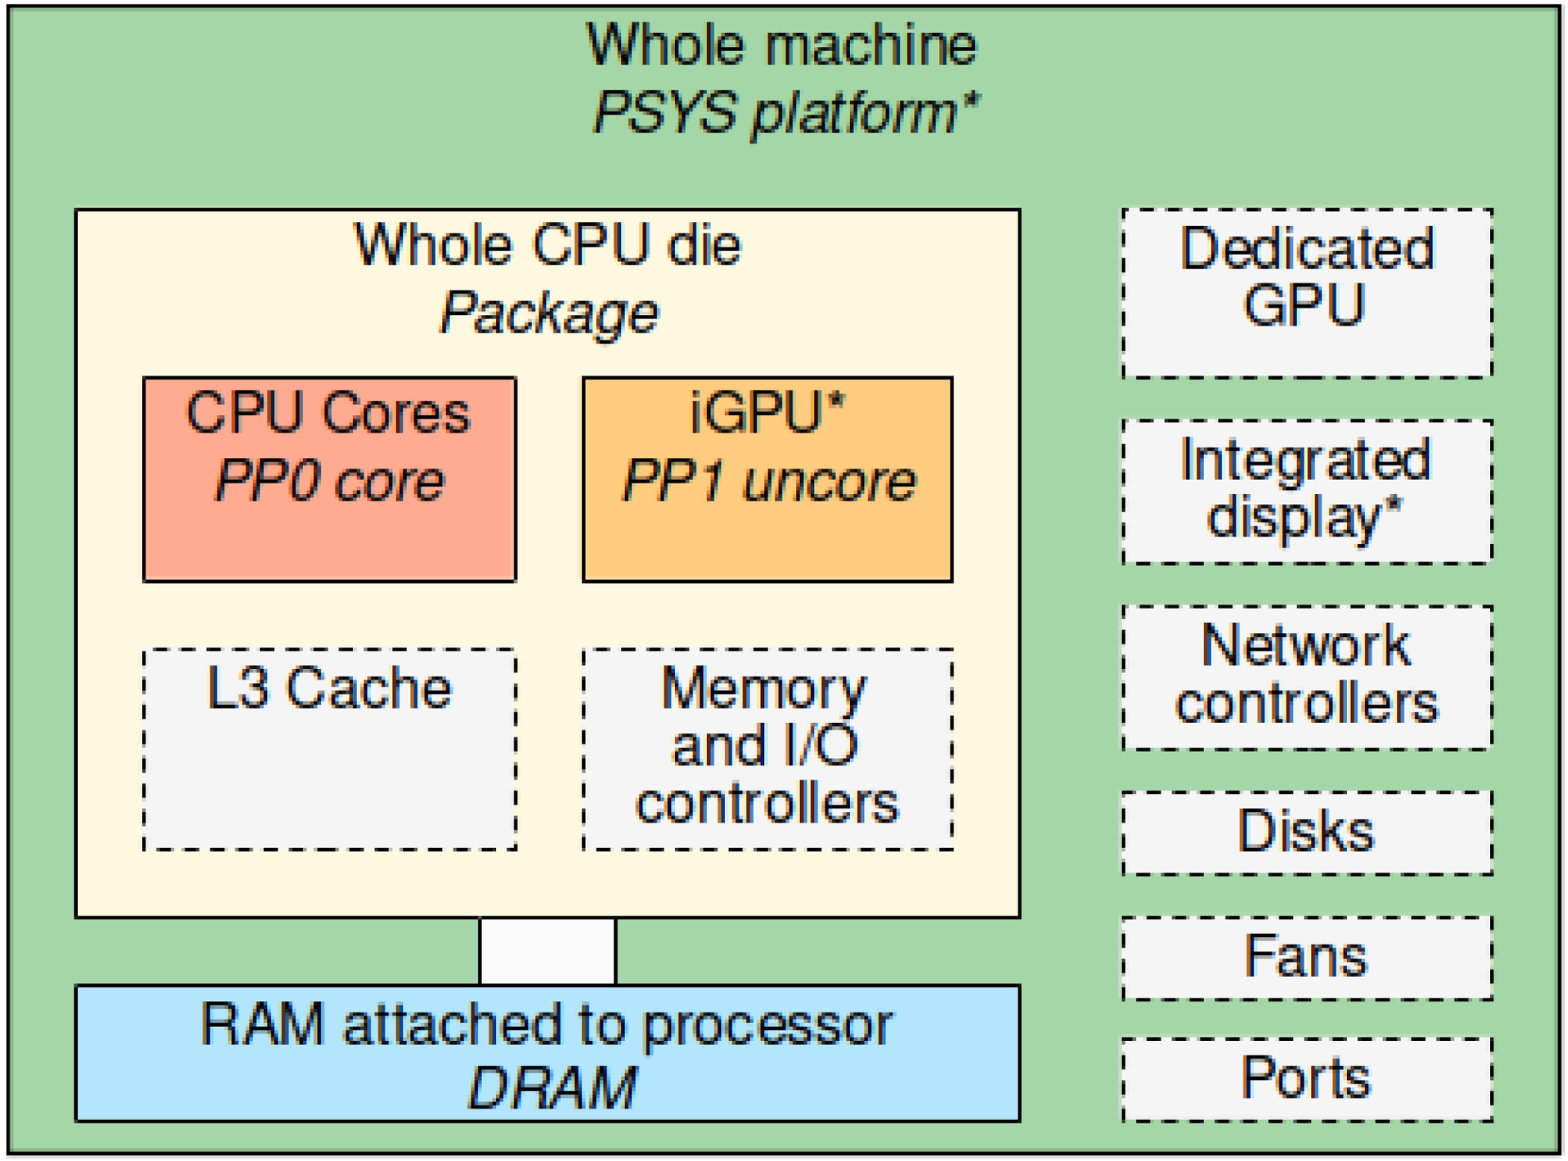
\includegraphics[width=0.7\textwidth]{Figures/rapl_domains.png}
    %\decoRule
    \caption[Rapl domains]{Hierarchy of possible RAPL domains and their corresponding hardware components. Domain names are in italic, and grayed items do not form a domain on their own, items with an asterisk are not present on servers\parencite{raffin2024dissecting}.}
    \label{fig:rapl_domains}
\end{figure}

RAPL provides hardware counters to read the energy consumption (and set power limits) for each domain. The energy consumption is measured in terms of processor-specific "energy units" (e.g. 61$\mu$J for Haswell and Skylake processors). The counters are exposed to the operating system through model-specific registers (MSRs) and are updated approximately every millisecond. The main advantages of RAPL are that no external powermeters are required, nor a privileged access to the BMC (which could be used to power off the server). RAPL is more accurate than any untuned statistical estimation model.

Various measurement methods can be used to extract RAPL measurements. In a detailed comparison, Raffin et al\parencite{raffin2024dissecting} outline their individual features and tradeoffs, which are summarize in figure~\ref{fig:rapl_interfaces_tradeoffs}:
\begin{itemize}
    \item The \textbf{Model-Specific Register (MSR)} interface provides low-level access to RAPL energy counters but is complex and hardware-dependent. Developers must manually determine register offsets and unit conversions based on processor model and vendor documentation. This method lacks safeguards, requires deep processor knowledge, and is error-prone, with incorrect readings difficult to detect. Although read-only access poses no risk to system stability, MSRs expose sensitive data and are thus restricted to privileged users (e.g., \texttt{root} or \texttt{CAP\_SYS\_RAWIO}). Fine-grained access control is not supported natively, though the \texttt{msr-safe} module offers limited mitigation.
    \item The \textbf{Power Capping (powercap)} framework is a high-level Linux kernel interface that exposes RAPL energy data through the sysfs filesystem, making it accessible from userspace. It simplifies energy measurements by automatically handling unit conversions and domain discovery, requiring minimal hardware knowledge. Though domain hierarchy can be confusing (especially with DRAM domains appearing nested under the package domain) powercap remains user-friendly and scriptable. It supports fine-grained access control via file permissions and offers good adaptability to hardware changes, provided the measurement tool doesn't rely on hard-coded domain structures.
    \item The \textbf{perf-events} subsystem provides a higher-level Linux interface for accessing RAPL energy counters as counting events. It supports overflow correction and requires less hardware-specific knowledge than MSR. Each RAPL domain must be opened per CPU socket using \texttt{perf\_event\_open}, and values are polled from userspace. While it lacks a hierarchical structure like powercap and may be harder to use in certain languages or scripts, it remains adaptable and robust across different architectures. Fine-grained access control is possible via kernel capabilities or \texttt{perf\_event\_paranoid} settings. 
    \item \textbf{eBPF} enables running custom programs in the Linux kernel, and in this context, it is used to directly read RAPL energy counters from within kernel space, potentially reducing measurement overhead by avoiding user-kernel context switches. The implementation attaches an eBPF program to a CPU clock event, using \texttt{perf\_event\_open} to access energy counters and buffering results for userspace polling (is visualized in figure~\ref{fig:rapl_perf_eBPF}).While offering the same overflow protection as regular \texttt{perf-events}, this approach is significantly more complex, prone to low-level errors (especially in C), and requires elevated privileges (\texttt{CAP\_BPF} or \texttt{root}). It also lacks portability, as it demands manual adaptation to kernel features and domain counts, limiting its maintainability across systems.
\end{itemize}
\begin{figure}[H]
    \centering
    \begin{subfigure}{0.48\textwidth}
        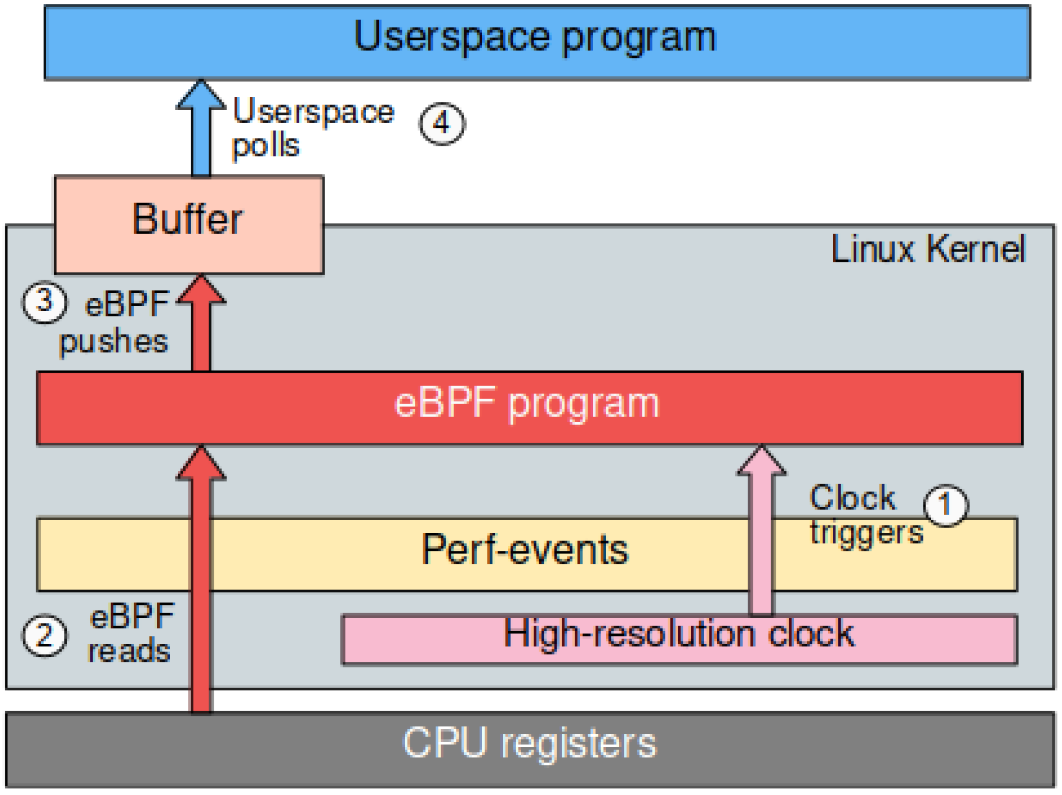
\includegraphics[width=\textwidth]{Figures/rapl_perf_eBPF.png}
        \caption[RAPL perf-event eBPF mechanism]{RAPL perf-event eBPF mechanism}
        \label{fig:rapl_perf_eBPF}
    \end{subfigure}
    \hfill
    \begin{subfigure}{0.48\textwidth}
        \vspace{1.5em}
        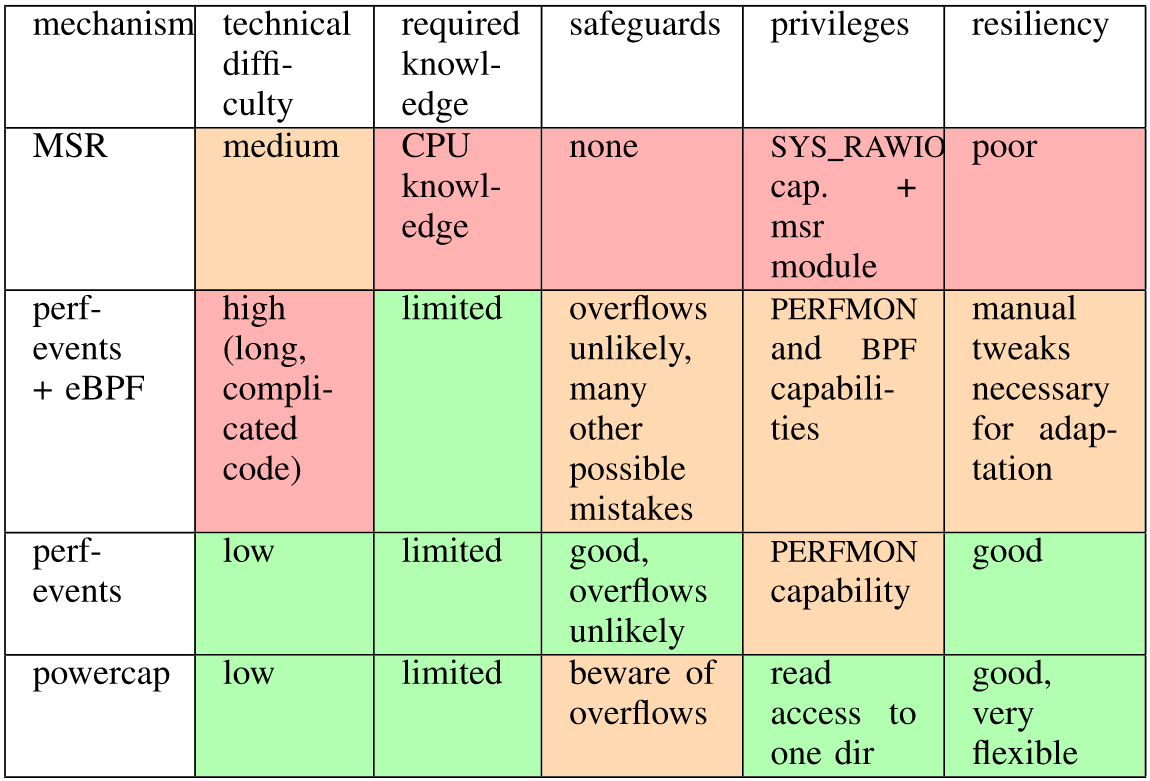
\includegraphics[width=\textwidth]{Figures/rapl_interfaces_tradeoffs.png}
        \caption[RAPL measurement mechanisms comparison]{RAPL measurement mechanisms comparison}
        \label{fig:rapl_interfaces_tradeoffs}
    \end{subfigure}
    \caption[RAPL measurements: eBPF and comparison]{RAPL measurements: eBPF and comparison\parencite{raffin2024dissecting}}
    \label{tab:measurement_mechanisms}
\end{figure}
In their research, Raffin et al conclude that all four mechanisms have small or negligible impact on the running time of their benchmarks. Based on their findings, formulate the following recommendations:
\begin{itemize}
    \item Measuring frequencies should be adapted to the state of the node, preventing high measurement overhead, due to a reduction in time spent in low-power states. Under heavy load, a highfrequencay can be used in order to capture more information.
    \item \texttt{perf-events} is the overall recommeded measurement method with good efficiency, latency and overflow protection. Powercap is less efficient, but provides a simpler sysfs API.
    \item Even though \texttt{perf-events} and eBPF-measurement method seems to be the most energy-efficient, it is not recommended in light of its complexity. For the same reason, the MSR method is not recommeded, as it raises complexity while counter-intuitively being slower than \texttt{perf-events}
\end{itemize}

\subsubsection{Validation}
\label{sec:raplvalidation}
Since its inception, RAPL has been subject of various validation studies, with the general concensus that it's accuracy could be considered "good enough"\parencite{raffin2024dissecting}. Notable works are Hackenberg et al, that in 2013 found RAPL accurate but missing timestamps\parencite{hackenberg2013power}, and in 2015 noticed a major improvement to RAPL accuracy, after Intel switched from a modeling approach to actual measurements for their Haswell architecture\parencite{hackenberg2015energy}. Desrochers et al concluded in a 2016 RAPL DRAM validation study\parencite{desrochers2016validation} that DRAM power measurement was reasonably accurate, especially on server-grade CPUs. They also found measurement quality to drop when measuring and idling system. Khan et al\parencite{khan2018rapl}

A critical point in the RAPL validation was the introduction of the Alder Lake architecture, marking Intel's first heterogeneous processor, combining two different core architectures from the Core and Atom families (commonly referred to as P-Cores and E-cores) to improve performance and energy efficiency. While this heterogenity can improve performance and energy efficiency, it also increases complexity of scheduling decisions and power saving mechanisms, adding to the already complex architecture, featuring per-core Dynamic Voltage and frequency Scaling (DVFS), Idle states and Power Limiting / Thermal Protection.



xxxxxxxxxxxxxxxxxxxxxxx \parencite{fahad2019comparative}(2019) ???????? (NO, ALDER LAKE WAS 2021)
BUT CHECK IT OUT ANYWAY
maybe include \parencite{alt2024experimental} (RECENT DRAM VALIDATION)



Schöne et al\parencite{schone2024energy} found RAPL in the Alder Lake architecture to be generally consistent with external measurements, but exhibiting lower accuracy in low power scenarios. The following figure~\ref{fig:rapl_vs_PSU_validation} shows these inaccuracies, albeit tested on a conusmer-grade Intel Core i9-12900K processor measured at the base frequency of 0.8GHz.
\begin{figure}[ht]
    \centering
    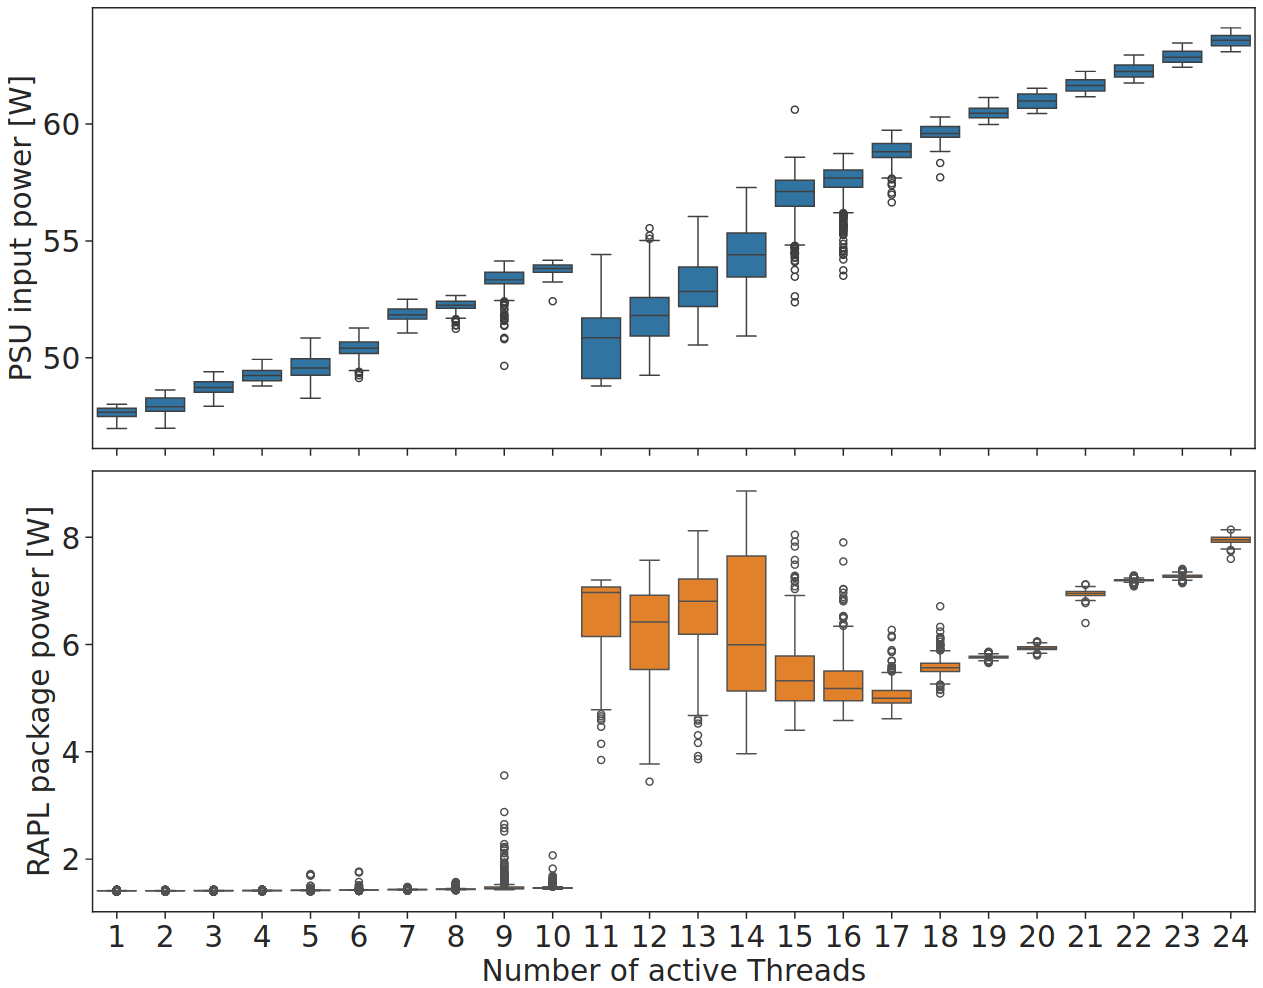
\includegraphics[width=0.7\textwidth]{Figures/rapl_vs_PSU_validation.png}
    %\decoRule
    \caption[RAPL validation: CPU vs. PSU]{RAPL and reference power consumption sampled at 100 ms / 50 ms intervals respectively. Double precision matrix multiplication kernel at 0.8GHz running for 60s each at increasing number of active threads\parencite{schone2024energy}.}
    \label{fig:rapl_vs_PSU_validation}
\end{figure}

\subsubsection{Limitations and issues}
\label{sec:rapllimitations}
Several limitations of RAPL were noticed in various research works. Since RAPL is continually improved by Intel as new Processors are released, some of these issues have since been improved or entirely solved. 

\begin{itemize}
    \item \textbf{Register overflow: }The 32-bit register can experience an overflow error\parencite{khan2018rapl, raffin2024dissecting}. This can be mitigated by sampling more frequently than the register takes to overflow. This interval can be calculated using the following equation: 
    \begin{equation}
        t_{\text{overflow}} = \frac{2^{32} \cdot E_u}{P}
    \end{equation}
    Here, $E_u$ is the energy unit used (61$\mu$J for haswell), and $P$ is the power consumption. On a Haswell processor consuming 84W, an overflow would occur every 52 minutes. Intel acknowledges this in the official documentation, stating that the register has a \textit{wraparound time of around 60 seconds when power consumption is high}\parencite{intel-sdm}
    This is solvable with a simple correction, provided that the measurement interfals are small enough: For two successive measurements $m_{\text{prev}}$ and $m_{\text{current}}$, the actual measured difference is given by
    \begin{equation}
        \Delta m =
        \begin{cases}
        m_{\text{current}} - m_{\text{prev}} + C & \text{if } m_{\text{current}} < m_{\text{prev}} \\
        m_{\text{current}} - m_{\text{prev}} & \text{otherwise}
        \end{cases}
    \end{equation}
    where C is a correction constant that depends on the chosen mechanism:
    
    \begin{table}[h]
        \small
        \begin{tabular}{|p{4cm}|p{9cm}|}
            \hline
            \textbf{mechanism} & \textbf{constant C}\\
            \Xhline{1.5pt}
            MSR & \texttt{u32::MAX} i.e. $2^{32} - 1$\\
            \hline
            perf-events & \texttt{u64::MAX} i.e. $2^{64} - 1$\\
            \hline
            perf-events with eBPF & \texttt{u64::MAX} i.e. $2^{64} - 1$\\
            \hline
            powercap & value give by the file \texttt{max\_energy\_uj} in the sysfs folder for the RAPL domain\\
            \hline
        \end{tabular}
        \caption[RAPL overflow correction constant]{RAPL overflow correction constant}
        \label{tab:RAPL_overflow_correction_constant}
    \end{table}

    \item \textbf{DRAM Accuracy: }DRAM Accuracy can only reliably be used for the Haswell architecture\parencite{desrochers2016validation, khan2018rapl}, and may still exibit a constant power offset.
    \item \textbf{Unpredictable Timings: }While the Intel documentation states that the RAPL time unit is 0.976ms, the actual intervals may vary. This is an issue since the measurements do not come with timestamps, making precise measurements difficult\parencite{khan2018rapl}. Several coping mechanisms have been used to mitigate this, notably \textit{busypolling} (busypolling the counter for updates, significantly compromizing overhead in terms of time and energy\parencite{hahnel2012measuring}), \textit{supersampling} (lowering the sampling interval, increasing overhead and occasionaly creating duplicates that need to be filtered\parencite{khan2018rapl}), or \textit{high frequency sampling} (\textit{lowering} the sampling rate when the resulting data is still sufficient\parencite{servat2016detailed}).
    \item \textbf{Lower idle power accuracy: } When measuring an idling server, RAPL tends to be less accurate\parencite{schone2024energy, desrochers2016validation}.
    \item \textbf{Side-channel attacks: } While the update rate of RAPL is usually 1ms, it can get as low as 50 $\mu$s for the PP0 domain (processor cores) on desktop processors\parencite{schone2024energy}. This can be used to retrieve processed data in a side channel attack (coined "Platypus")\parencite{lipp2021platypus, schone2024energy}. 
    
    To mitigate this issue while retaining RAPL functionality, Intel implements a filtering technique via the \texttt{ENERGY\_FILTERING\_ENABLE}\parencite[Table 2-2]{intel20023} entry, or when \textit{Software Guard Extension (SGX)} is activated in the BIOS. This filter adds random noise to the reported values (vizualized in Figure~\ref{fig:rapl_platypus_filtering}). This can be seen For the PP0 domain, this raises the temporal granularity to about 8ms. While this does not affect the average power consumption, point measurement power consumption can be affected. Figure~\ref{fig:rapl_filter_granularity_loss} shows the effect of the filter, clearly indicating the loss granularity resulting from the activation of the filter. In a 2022 article, Tamara\parencite{greencoding_rapl_sgx} found a surprising higher mean with the filter activated and deemed filtered RAPL energy data unusable. In a more elaborate experiment in 2024, Schöne et al did not encounter these inaccuracies anymore.

    \begin{figure}[H]
        \centering
        \begin{subfigure}[t]{0.6\textwidth}
            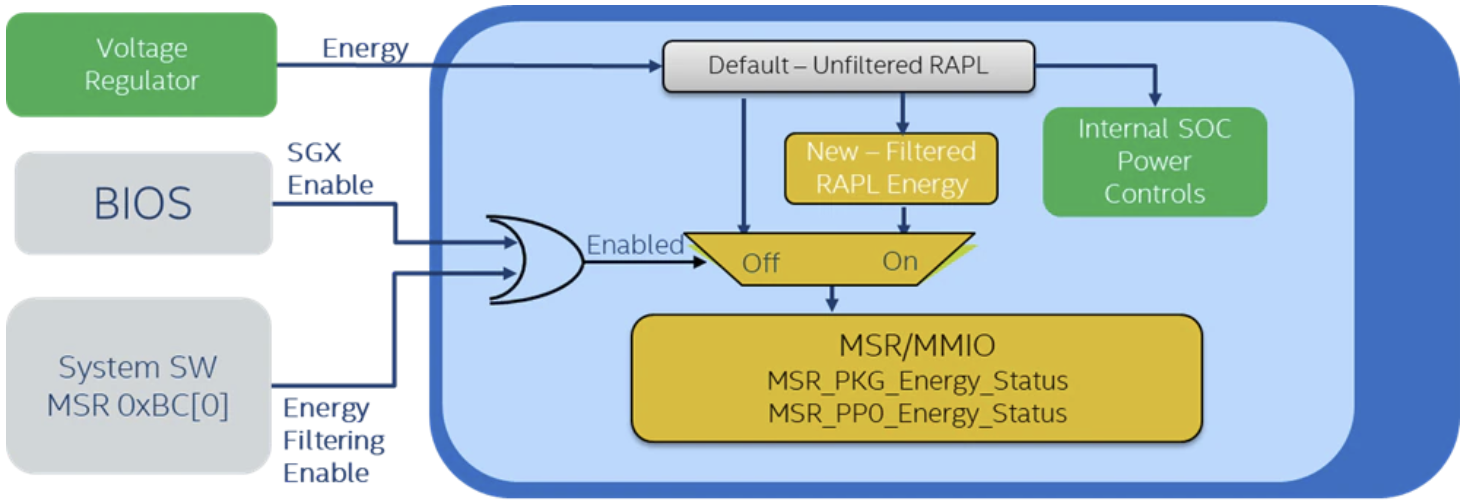
\includegraphics[width=\textwidth]{Figures/rapl_platypus_filtering.png}
            \caption{RAPL energy filtering\parencite{intel_rapl_guidance}}
            \label{fig:rapl_platypus_filtering}
        \end{subfigure}
        \begin{subfigure}[t]{0.48\textwidth}
            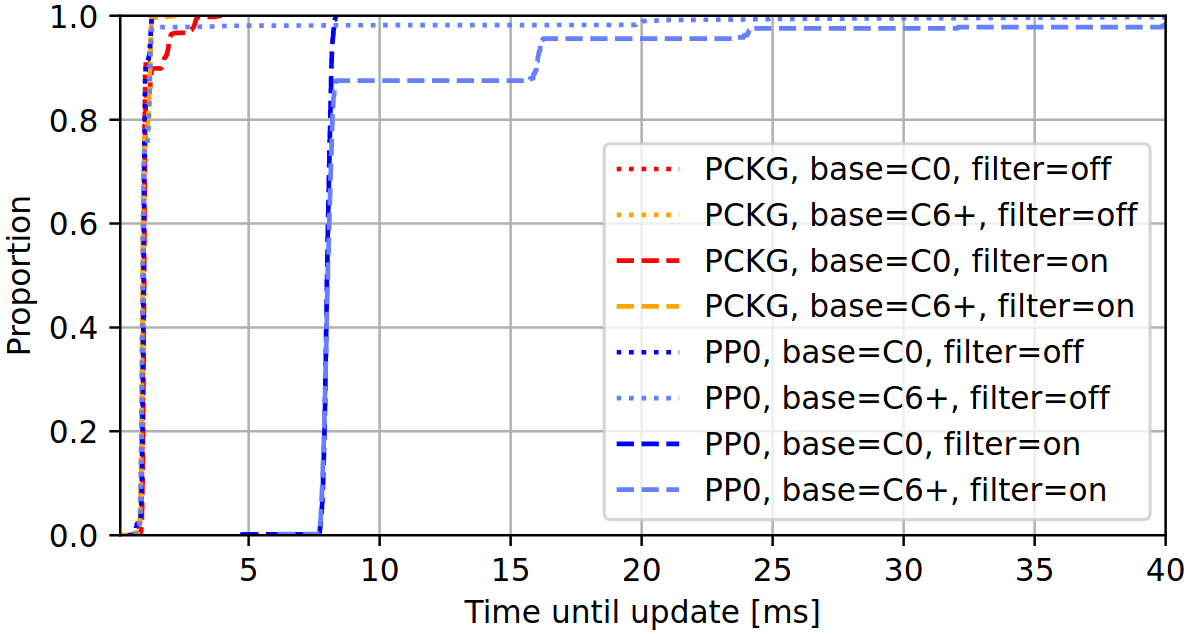
\includegraphics[width=\textwidth]{Figures/rapl_filter_granularity_loss_time.png}
            \caption{Distribution of time between updates: With an enabled filter, the PP0 domain only provides updates every 8 ms, otherwise RAPL values are updated every 1 ms. If the load is too low, some updates might be skipped, e.g., the next update for PP0 and an enabled filter is at 16 ms.}
            \label{fig:rapl_filter_granularity_loss_time}
        \end{subfigure}
        \hfill
        \begin{subfigure}[t]{0.48\textwidth}
            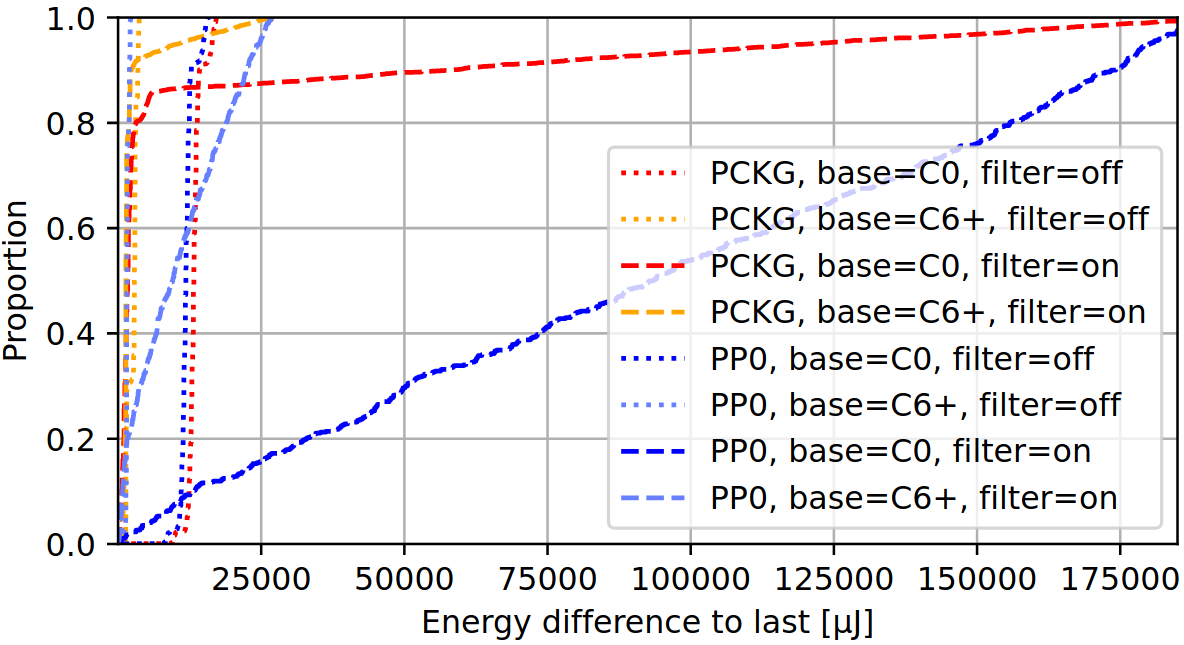
\includegraphics[width=\textwidth]{Figures/rapl_filter_granularity_loss_energy.png}
            \caption{The minimal increase of a measurement is 1 energy unit of 61.035~$\mu$J. Enabling the filter leads to a significant influence on measurements for the PP0 domain and a measurable influence on PCKG measurements.}
            \label{fig:rapl_filter_granularity_loss_energy}
        \end{subfigure}
        \caption[Observable loss of granularity caused by the activation of \texttt{ENERGY\_FILTERING\_ENABLE}]{Observable loss of granularity caused by the activation of \texttt{ENERGY\_FILTERING\_ENABLE}\parencite{schone2024energy}}
        \label{fig:rapl_filter_granularity_loss}
    \end{figure}
\end{itemize} 

\section{Server Power models}
In the absence of actual power data, power consumption models can be formulated that essentially map variables (such as CPU, Memory utilization) related to a server's state to its power consumption. 
Due to the strong correlation between CPU uzilization and server power, a great number of models use CPU metrics as the only indicator of server power. Fan et al\parencite{fan2007power} proposed a linear interpolation between idle power and full power, which they further refine into a non-linear form, with a parameter $\gamma$ to be fitted to minimize mean square error. Similar research was done to further reduce error by introducting more complex non-linear models, such as Hsu and Poole\parencite{hsu2011power}, who studied the SPECpower\textunderscore ssj2008-dataset of systems released between December 2007 and August 2010, and suggested the adaptation of two non-linear terms:
\begin{equation}
    P_{\text{server}} = \alpha_0 + \alpha_1 u_{\text{cpu}} + \alpha_2 \left( u_{\text{cpu}} \right)^{\gamma_0} + \alpha_3 \left( 1 - u_{\text{cpu}} \right)^{\gamma_1}
\end{equation}

While models like these might work well when custom-fitted to specific, multi-purpose servers, they have since been surpassed by the more common approach of modelling server power is to consider it an assembly of its components, such as Song et al\parencite{song2013unified} propose as:
\begin{equation}
    P_{\text{server}} = P_{\text{cpu}} + P_{\text{memory}} + P_{\text{disk}} + P_{\text{NIC}} + C
\end{equation}
, where C denotes the server's base power, which includes the power consumption of other components (regarded as static). This approach can easily be extended to include various other components such as GPUs, FPGAs or other connected components.


....




In a systematic review cloud servers power models, Lin et al\parencite{lin2020taxonomy} state that the common way


\section{Power data collection}

see Lin et al for overview -> instruments / dedicated aquisition system / software monitoring and calculation / simulation

\subsection{CPU}

\subsection{Memory}

\subsection{Storage}

\subsection{Networking}

\section{Container energy estimation based on hardware power estimation}
% see lin et al

\section{Tools}
\subsection{RAPL-based tools}
\label{sec:rapltools}
\begin{itemize}
    \item \parencite{jay2023experimental} An experimental comparison of software-based power meters (focus on CPU / GPU)
    \item \parencite{kavanagh2019rapid} Rapid and accurate energy models through calibration with IPMI and RAPL
    \item \parencite{scaphandre_documentation} Scaphandre. Does not handle overflows correctly (https://github.com/hubblo-org/scaphandre/issues/280)
    \item \parencite{fieni2020smartwatts} Smartwatts: Self-Calibrating Software-Defined Power Meter for containers
    \item \parencite{joularjx} JoularJX: jaba-based agent for power monitoring at the code level
    \item \parencite{kepler_energy}: KEPLER
    \item \parencite{aipowermeter}: "AI power meter": Library to measure energy usage of machine learning programs, uses RAPL for CPU and nvidia-smi for GPU
    \item \parencite{codecarbon} CodeCarbon: Python package, estimates GPU + CPU + RAM: uses pynvml, ram RATIO (3W for 8G) and RAPL. According to Raffin2024, this tool does not account for the MSR overflow: https://github.com/mlco2/codecarbon/issues/322 -> apparently fixed now
    \item \parencite{powertop}: powertop
    \item \parencite{greencodingdocs}: Green metrics tool: measuring energy and CO2 consumption of software through a software life cycle anslysis (SLCA): Metric providers: RAPL, IPMI, PSU, Docker, Temperature, CPU, ... (sone external devices)
    
    according to raffin2024: simplified versions of scaphandre and codecarbon hhve 3\%, 0.5\% overhead at 10Hz
    according to \parencite{jay2023experimental}, the full versions have between 2 and 7\% at 1Hz.

\parencite{fieni2024powerapi}: PowerAPI: Python framework for building software-defined power
\end{itemize}
\begin{comment}
- multiple papers have tried to attribute component-level 
\end{comment}




\section{"data fusion of power data and cpu metrics}
- Estimating the consumption of a single function has been proven to be possible in 2012: M. Hähnel, B. Döbel, M. Völp, and H. Härtig, “Measuring energy consumption for short code paths using RAPL,”, \parencite{hahnel2012measuring}



% \section{Introduction}
% \begin{itemize}
%     \item Motivation for accurate energy consumption measurement in containerized environments
%     \item Scope of this chapter
%     \item Structure of the chapter
% \end{itemize}

% \section{Validation of Energy Measurement Methods}
% \subsection{Overview of Measurement Interfaces}
% \begin{itemize}
%     \item Intel RAPL (Running Average Power Limit)
%     \item BMC Interfaces (e.g., Redfish, IPMI)
%     \item Wall Power Meters (e.g., smart PDUs, power sockets)
% \end{itemize}

% \subsection{Cross-Validation Studies}
% \begin{itemize}
%     \item Comparison between RAPL, BMC, and Wall Power
%     \item Known inaccuracies and calibration techniques
%     \item Resolution and update frequency
% \end{itemize}

% \subsection{Limitations and Challenges}
% \begin{itemize}
%     \item Hardware-specific behaviors
%     \item Temporal resolution vs accuracy
%     \item External factors (thermal throttling, BIOS settings)
% \end{itemize}

% \section{System-Level Energy Measurement Tools}
% \subsection{Overview of Common Tools}
% \begin{itemize}
%     \item PowerTOP
%     \item ipmitool and Redfish CLI tools
%     \item perf, turbostat, msr-tools
% \end{itemize}

% \subsection{Capabilities and Use Cases}
% \begin{itemize}
%     \item Server power monitoring
%     \item Power modeling and estimation
%     \item Energy-aware scheduling (non-containerized)
% \end{itemize}

% \subsection{Strengths and Limitations}
% \begin{itemize}
%     \item Overhead and granularity
%     \item Portability across hardware
%     \item Integration with monitoring stacks (e.g., Prometheus)
% \end{itemize}

% \section{Taxonomy of Energy Measurement Approaches}
% \subsection{Measurement Dimensions}
% \begin{itemize}
%     \item Direct vs Indirect Measurement
%     \item Real-time vs Offline Analysis
%     \item Hardware-Level vs OS-Level vs Application-Level
%     \item Static Models vs Dynamic Instrumentation
% \end{itemize}

% \subsection{Attribution Granularity}
% \begin{itemize}
%     \item Node-level, Process-level, Container-level
%     \item Component breakdown (CPU, memory, I/O, network)
% \end{itemize}

% \section{Container-Level Energy Consumption Measurement}
% \subsection{Challenges in Container Environments}
% \begin{itemize}
%     \item Resource sharing and cgroup isolation
%     \item Transient workloads and short-lived containers
%     \item Scheduler noise and runtime variability
% \end{itemize}

% \subsection{Strategies for Energy Attribution}
% \begin{itemize}
%     \item Per-process accounting and aggregation
%     \item Performance counters and sampling
%     \item Machine learning and model-based inference
% \end{itemize}

% \subsection{Tools and Frameworks}
% \begin{itemize}
%     \item \textbf{Kepler}: BPF-based metrics and ML models
%     \item \textbf{Scaphandre}: powercap interface and Prometheus export
%     \item \textbf{PowerAPI}, \textbf{PowerVisor}, other academic tools
% \end{itemize}

% \subsection{Evaluation and Comparison}
% \begin{itemize}
%     \item Accuracy and validation methods
%     \item Measurement overhead
%     \item Deployment complexity and scalability
% \end{itemize}

% \section{Use Cases and Evaluation Criteria}
% \subsection{Real-World Applications}
% \begin{itemize}
%     \item Data center energy reporting
%     \item Cost-aware scheduling and autoscaling
%     \item SLA monitoring and anomaly detection
% \end{itemize}

% \subsection{Evaluation Dimensions}
% \begin{itemize}
%     \item Precision and granularity
%     \item Resource overhead
%     \item Hardware and software portability
%     \item Ease of integration
% \end{itemize}

% \section{Limitations and Open Research Questions}
% \begin{itemize}
%     \item Lack of standardization and benchmarks
%     \item Difficulty in attributing non-CPU power usage
%     \item Trade-offs between overhead and accuracy
%     \item Need for reproducibility across diverse platforms
% \end{itemize}

% \section{Industrial Practices and Emerging Trends}
% \begin{itemize}
%     \item Open Compute Project (OCP) standards
%     \item Google, Microsoft, Amazon energy-aware systems (if publicly available)
%     \item Sustainability metrics and reporting frameworks (e.g., Scope 2 emissions)
% \end{itemize}

% \section{Summary}
% \begin{itemize}
%     \item Recap of covered measurement methods and tools
%     \item Key insights into container-level energy measurement
%     \item Motivation for the approach used in this thesis
% \end{itemize}
